\section{Introduction}

This laboratory's main objective is to conceive a Bandpass filter circuit using OP-AMP. The circuit is composed of three parts, the first part cuts low frequencies, the second part amplifies the signal, and the third part cuts high frequencies, this circuit can be seen in figure \ref{Fig1: circuit}.

To build this circuit we have to maximize the merit. The merit of the work is given by:
\begin{equation}
    Merit = \dfrac{voltageGain \times bandwidth}{Cost (voltage gain deviation + central frequency deviation + 10^{-6})}
\end{equation}

We also need to build the circuit as cheap as we can. Both \SI{1}{\kilo\ohm}, in a resistance, and \SI{1}{\micro\farad}, in a capacitor, cost 1 Monetary Unit (MU). Other elements used are transistors and diodes which costs 0.1 MU per unit.
With this price table, we can compute the cost
\begin{equation}
    Cost = N_{transistors}*0.1+N_{diodes}*0.1+N_{Resistances}*1+N_{Capacitors}*1
\end{equation}

In the amplifier part of the circuit, we will be using a $\mu A741$ OP-AMP (Operational Amplifier) and two resisters, this circuit should be connected so that there is negative feedback to ensure that the positive and negative inputs of the OP-AMP have the same voltage. The low-frequency filter is composed of a capacitor and a resistor connected to the ground; the high frequency is composed of a resistor and a capacitor connected to the ground. The circuit is depicted in figure \ref{Fig1: circuit}.

\begin{figure}[h] 
\centering
\includegraphics[width=0.6\linewidth]{t5.pdf}
\caption{Circuit Concept.}
\label{Fig1: circuit}
\end{figure}

The ciruit tested in the laboratory ca be seen in the following figure:

\begin{figure}[h] 
\centering
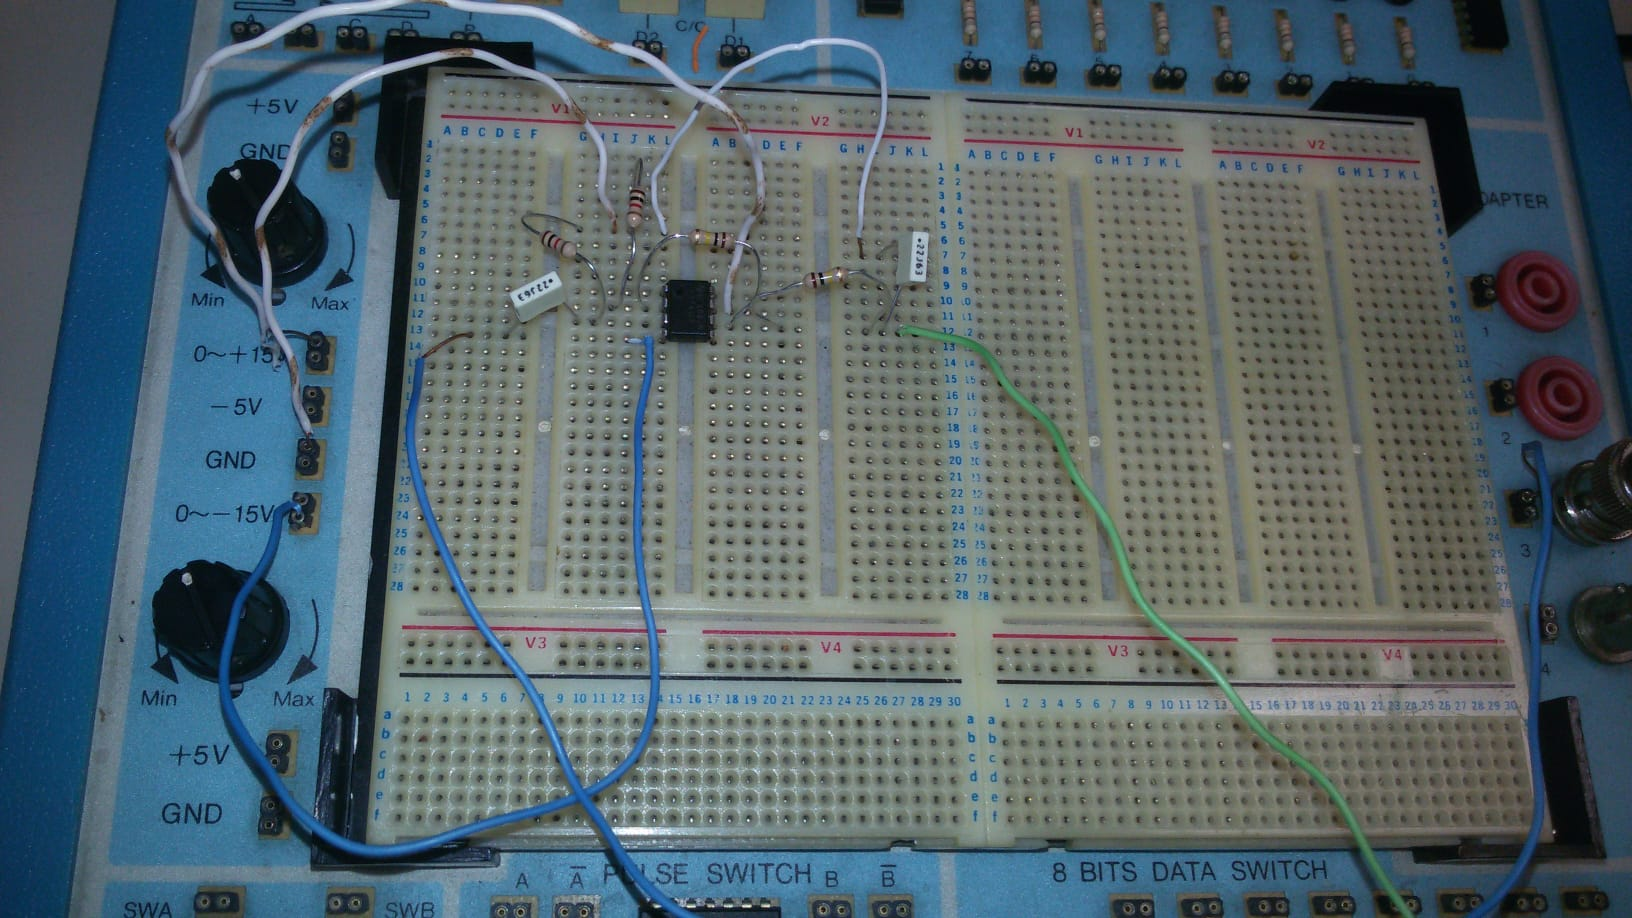
\includegraphics[width=0.6\linewidth]{Lab_Circuit.jpeg}
\caption{Circuit tested in the Laboratory.}
\label{Fig1.1: labcircuit}
\end{figure}

Plots and results are shown again after the $\ref{sec:analysis}^{nd}$ and $\ref{sec:simulation}^{rd}$ sections for an easier comparison.
